\documentclass[journal]{IEEEtran}

\usepackage{cite}
\usepackage{amsmath,amssymb,amsfonts}
\usepackage{graphicx}
\usepackage{booktabs}
\usepackage{array}
\usepackage{tikz}
\usetikzlibrary{arrows.meta,positioning}
\usepackage{url}

\graphicspath{{figures/}}

\begin{document}

\title{Metric Mismatch in Frequency-Selective Personal-Audio Limiting: A-Weighting versus {BS.1770}}

\author{Yashwini~Krishna~Murthy and Bhavya~Shri%
\thanks{The authors are with the Department of Computer Science and Engineering, Vellore Institute of Technology, Chennai, India (e-mail: yashwini.krishna2024@vitstudent.ac.in).}}

\markboth{IEEE Student Research Paper, VIT Chennai}%
{Murthy and Shri: Metric Mismatch in Frequency-Selective Personal-Audio Limiting}

\maketitle

\begin{abstract}
Conventional personal-audio limiters reduce listening level by applying one gain to every frequency. A-weighted exposure and programme loudness do not weight the spectrum in the same way, so it is reasonable to ask whether cutting some bands more than others can lower an exposure metric at the same loudness. This paper tests that question with a three-band digital processor: a complementary Linkwitz--Riley split at 300\,Hz and 4\,kHz, a low-band shelf of $-12$\,dB with harmonic fill from 80 to 400\,Hz, an A-weighted mid-band compressor, and a mild high-band envelope gain. On 20 clips (16 Freesound recordings and four synthetic signals) we compare the processor with frequency-flat gain under two matching rules. At matched BS.1770 loudness (LUFS), the proposed system's digital A-weighted $L_{Aeq}$ proxy is on average 1.17\,dB higher than flat gain. The matched-loudness exposure hypothesis is therefore not supported. The gap is largest on bass-heavy material (about $+1.6$ to $+2.7$\,dB on real bass loops). Vocals, speech, and short transients are essentially tied. The reason is straightforward: A-weighting already discards most energy near 40\,Hz, so removing sub-bass lowers LUFS much more than $L_{Aeq}$, and flat gain must then cut the midrange to match loudness. At matched $L_{Aeq}$ the proposed output is correspondingly quieter. All levels in this study are digital-domain proxies, not calibrated ear-level SPL.
\end{abstract}

\begin{IEEEkeywords}
Audio signal processing, A-weighting, K-weighting, dynamic range compression, frequency allocation, frequency-selective limiting, loudness, multiband processing, virtual bass.
\end{IEEEkeywords}

\section{Introduction}

Personal listening devices can deliver high playback levels for long periods. The World Health Organization and ITU-T Recommendation H.870 treat this as a cumulative A-weighted sound-dose problem and give device makers a framework for tracking exposure \cite{H870,WHO2021,Levey2011,Portnuff2011}. H.870 specifies \emph{how much} dose to allow. It does not pick a signal-processing algorithm. Device algorithms nonetheless exist: broadband dynamic-range control for H.870 listening \cite{Chen2023}, time-weighted-average (TWA) limiting with optional multiband companding \cite{US9980028}, and headset dosimetry that applies frequency-flat gain \cite{US6826515}. The standard is silent on allocation; that is not the same as ``no algorithm exists.''

The usual engineering response is a broadband limiter or automatic gain control \cite{Giannoulis2012}: when an exposure estimate exceeds a threshold, apply one scalar $G<1$ to the whole signal. That is easy to implement and it does reduce an A-weighted metric. It is also crude. Equal-loudness contours \cite{FletcherMunson1933,ISO226} show that hearing sensitivity is strongly frequency-dependent, so a flat cut changes bass, midrange, and treble by different perceptual amounts. Multiband compression and virtual-bass methods already exist as separate tools. What is missing is a direct test: if those tools are combined into an exposure-oriented limiter, do they beat ``turn everything down'' when exposure or loudness is matched?

That is the question of this paper. We ask:

\begin{quote}
\textit{Can frequency-selective gain allocation reduce an A-weighted digital exposure proxy more than conventional broadband attenuation at matched loudness, and preserve quality better at matched exposure?}
\end{quote}

We implement three systems on the same audio: the original clip, frequency-flat gain, and a three-band processor described in Section~\ref{sec:method}. We then match either LUFS or the digital $L_{Aeq}$ proxy and compare the other quantity. The ingredients are not new. The comparison is the contribution.

The result is mixed, and on the main hypothesis it is negative. At matched LUFS the proposed processor has a \emph{higher} digital $L_{Aeq}$ proxy than flat gain, by 1.17\,dB on average over 20 clips. Bass-heavy programme accounts for almost all of the difference. Speech, vocals, and short transients sit near a tie. Section~\ref{sec:results} shows why: the processor spends its budget on a band that A-weighting barely counts.

The rest of the paper is organised as follows. Section~\ref{sec:related} reviews related methods and states the gap. Section~\ref{sec:method} describes the processor as a design heuristic, not as a numerical solver. Section~\ref{sec:impl} records implementation and verification. Section~\ref{sec:setup} defines the experiment. Section~\ref{sec:results} reports the 20-clip comparison. Section~\ref{sec:limits} collects limitations in one place. Section~\ref{sec:conclusion} concludes.

\section{Related Work}
\label{sec:related}

\subsection{Exposure control}

H.870 defines an A-weighted sound-allowance model and discusses the difficulty of mapping a digital signal to ear-level pressure, which depends on transducer sensitivity and volume setting \cite{H870}. Device-side responses are typically volume caps, dose meters, or broadband automatic gain reduction \cite{Levey2011,Sulaiman2013,Chen2023}. Chen \emph{et al.} combine H.870 dose tracking, speaker frequency-response correction, and broadband DRC to lower SPL as allowance is used \cite{Chen2023}. US~6\,826\,515 is a headset dosimeter whose corrective gain is frequency-flat, so the chosen equalisation is preserved \cite{US6826515}; that is the baseline of this paper in patent form. US~9\,980\,028 is a TWA limiter that may use multiband companding to keep speech loudness while cutting RMS energy \cite{US9980028}. Those systems manage level, or allocate it for speech-headset intelligibility. They do not report a matched LUFS versus digital $L_{Aeq}$ comparison on music.

\subsection{Dynamic range control}

Digital compressors and limiters are well understood \cite{Giannoulis2012,Kates2008}. Multiband designs apply a separate envelope in each band and are usually tuned for tonal balance, broadcast loudness, or hearing-aid audibility---not for an exposure-versus-loudness comparison against a flat baseline. Multi-band hearing-protection processors \cite{Fathima2026} allocate gain across frequency to tame transients in speech and noise; they are adjacent, but they are not a matched LUFS/$L_{Aeq}$ test on music. ITU-R BS.1770 is the standard programme-loudness meter used here as a loudness stand-in \cite{BS1770}.

\subsection{Loudness perception}

ISO~226 equal-loudness contours \cite{ISO226} and excitation-pattern models \cite{Zwicker1961,ZwickerFastl1999,MooreGlasbergBaer1997,GlasbergMoore2002} explain why a flat gain change is not perceptually flat. This paper uses that fact as motivation. It does not implement a Zwicker or Moore--Glasberg loudness model. Integrated LUFS is the operational loudness measure.

\subsection{Virtual bass}

When a harmonic complex loses its fundamental, listeners can still hear a pitch at $f_0$ \cite{Schouten1940,Terhardt1974,Terhardt1979}. Loudspeaker virtual-bass systems exploit that residue pitch by synthesising harmonics when the driver cannot reproduce sub-bass \cite{BenTzur1999,Gan2001,Gan2004}. We use the same mechanism in the opposite direction: attenuate physical sub-bass and add harmonics in 80--400\,Hz. Residue pitch is not the same thing as preserved bass loudness, and we do not treat it as such.

\subsection{Gap}

Table~\ref{tab:gap} summarises the pieces. Frequency-selective tools for dose, hearing protection, and loudness already exist. What is scarce is a matched LUFS versus digital $L_{Aeq}$ test of a bass-first heuristic on music. That comparison is what this study provides. It does not introduce a new limiter architecture.

\begin{table}[!t]
\caption{Related methods versus this study. ``Matched test'' here means equal LUFS or equal digital $L_{Aeq}$ on music, for a bass-first frequency heuristic versus flat gain.}
\label{tab:gap}
\centering
\renewcommand{\arraystretch}{1.12}
\begin{tabular}{>{\raggedright\arraybackslash}p{0.20\columnwidth} c c c c c}
\hline
Approach & Exposure & Freq.\ adapt. & Loudness aim & Bass fill & Matched test \\
\hline
H.870-style dose limit \cite{H870} & Yes & No & No & No & No \\
Broadband limiter / PLD DRC \cite{Giannoulis2012,Chen2023} & Yes & No & Indirect & No & Baseline \\
Flat-gain headset dosimeter \cite{US6826515} & Yes & No & No & No & Baseline \\
TWA limiter + optional multiband \cite{US9980028} & Yes & Optional & Speech & No & No \\
Multiband DRC / hearing-aid compression \cite{Kates2008} & Partial & Yes & Partial & Rare & Rare \\
Multi-band hearing protection \cite{Fathima2026} & Yes & Yes & Speech & No & No \\
Virtual bass \cite{Gan2001} & No & Yes & Bass only & Yes & No \\
This work (bass-first heuristic) & Proxy & Yes & LUFS & Yes & Yes \\
\hline
\end{tabular}
\end{table}

\section{Proposed Method}
\label{sec:method}

\subsection{Design objective}

Let $x[n]$ be the input. A conventional limiter applies one gain
\begin{equation}
y[n] = G\, x[n], \qquad G < 1.
\label{eq:flat}
\end{equation}
We want a frequency-dependent alternative that, for a given loudness, yields a lower A-weighted digital exposure proxy than \eqref{eq:flat}. Preferentially cutting energy that contributes more to A-weighting than to loudness is the intended trade-off. Preferentially cutting energy that A-weighting already ignores is the failure mode.

This is a design objective, not a solved optimisation. We do not run a numerical solver for a constrained cost. The implementation is a fixed three-band heuristic built toward that trade-off.

\subsection{Architecture}

The signal is split at 300\,Hz and 4\,kHz, processed per band, summed, and passed through a fixed-ceiling peak limiter (Fig.~\ref{fig:block}):
\begin{equation}
y[n] = y_{\mathrm{L}}[n] + y_{\mathrm{M}}[n] + y_{\mathrm{H}}[n].
\end{equation}
The low band carries sub-bass, the mid band most speech and musical energy, and the high band many transients. Those cutoffs were chosen for the prototype. They were not optimised by a listening-test search.

\begin{figure*}[!t]
\centering
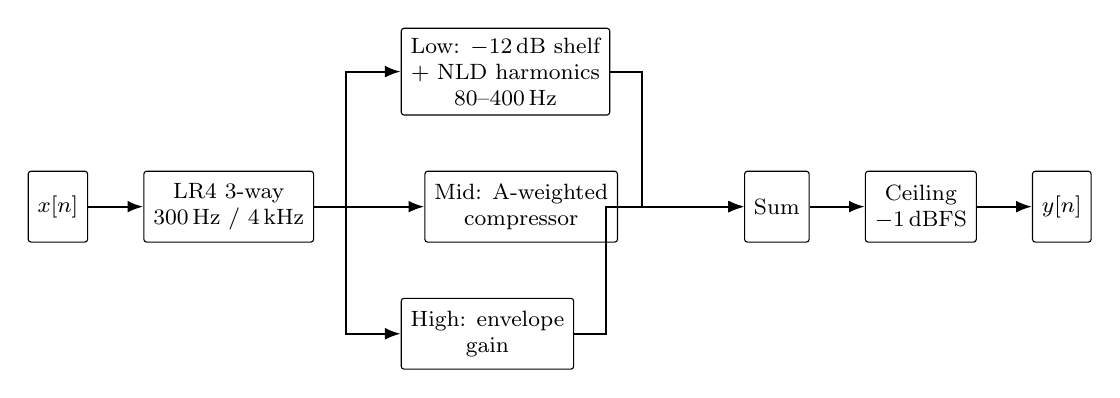
\begin{tikzpicture}[
  font=\footnotesize,
  box/.style={draw, align=center, inner sep=3.4pt, minimum height=9mm, rounded corners=1pt},
  arr/.style={-{Latex[length=2mm]}, thick}
]
\node[box] (x) {$x[n]$};
\node[box, right=7mm of x] (xo) {LR4 3-way\\$300$\,Hz / $4$\,kHz};
\node[box, above right=7mm and 11mm of xo] (lo) {Low: $-12$\,dB shelf\\+ NLD harmonics\\$80$--$400$\,Hz};
\node[box, right=14mm of xo] (mid) {Mid: A-weighted\\compressor};
\node[box, below right=7mm and 11mm of xo] (hi) {High: envelope\\gain};
\node[box, right=16mm of mid] (sum) {Sum};
\node[box, right=7mm of sum] (pk) {Ceiling\\$-1$\,dBFS};
\node[box, right=7mm of pk] (y) {$y[n]$};
\draw[arr] (x) -- (xo);
\draw[arr] (xo.east) -- ++(4mm,0) |- (lo.west);
\draw[arr] (xo) -- (mid);
\draw[arr] (xo.east) -- ++(4mm,0) |- (hi.west);
\draw[arr] (lo.east) -- ++(4mm,0) |- (sum.west);
\draw[arr] (mid) -- (sum);
\draw[arr] (hi.east) -- ++(4mm,0) |- (sum.west);
\draw[arr] (sum) -- (pk);
\draw[arr] (pk) -- (y);
\end{tikzpicture}
\caption{Three-band processor. The crossover is complementary. Per-band processing is a fixed heuristic, not a numerical optimiser.}
\label{fig:block}
\end{figure*}

\subsection{Low band}

A low shelf of $\beta = 10^{-12/20} \approx 0.25$ ($-12$\,dB) is applied around 100\,Hz. Harmonics are generated from the isolated sub-bass $x_{\mathrm{sub}}$ by a memoryless nonlinearity
\begin{equation}
x_{\mathrm{NLD}}[n] = a_2\, x_{\mathrm{sub}}^2[n] + a_3\, x_{\mathrm{sub}}^3[n]
\end{equation}
with $a_2=0.8$ and $a_3=0.35$, then band-pass filtered to 80--400\,Hz and mixed back. An earlier 160--300\,Hz harmonic window missed $2f_0$ and $3f_0$ for fundamentals near 40\,Hz. The wider window is used so that a 40\,Hz tone actually produces energy at 80 and 120\,Hz (Fig.~\ref{fig:harm}). Harmonic injection supports a residue pitch cue. It is not evidence that bass loudness is preserved.

\subsection{Mid band}

The mid band is compressed from an A-weighted envelope. If $e[n]$ is that envelope and
\begin{equation}
L[n] = 20\log_{10}(e[n]+\varepsilon) + L_{\mathrm{ref}},
\end{equation}
gain reduction of ratio $R=4$ is applied only when $L[n]$ exceeds a target of 78 (the same uncalibrated digital offset $L_{\mathrm{ref}}=94$ used in the exposure proxy):
\begin{equation}
g_{\mathrm{M}}[n] = 10^{-(1-1/R)\max(L[n]-L_{\mathrm{tgt}},0)/20}.
\end{equation}
Attack and release are 5\,ms and 50\,ms. The A-weighting filter is the IEC~61672 analog prototype \cite{IEC61672}, bilinearly transformed at 48\,kHz and normalised to 0\,dB at 1\,kHz. Inside 300\,Hz--4\,kHz, where this detector is used, the digital magnitude tracks the analytic curve to well under 0.2\,dB. Above about 8\,kHz the bilinear transform warps the response; that region is not used for mid-band detection (Fig.~\ref{fig:aw}).

\subsection{High band}

Content above 4\,kHz is scaled by a one-pole envelope $E[n]$:
\begin{equation}
y_{\mathrm{H}}[n] = x_{\mathrm{H}}[n]\cdot \frac{1}{1+\gamma \max(0, E[n]-T_{\mathrm{H}})},
\end{equation}
with $\gamma=0.5$ and $T_{\mathrm{H}}=-12$\,dBFS. This is transient-aware gain control. It is not a validated perceptual model.

\subsection{Crossover reconstruction}

Independent Butterworth low/band/high splits are not magnitude-complementary and can boost the sum near the cutoffs. The processor uses cascaded fourth-order Linkwitz--Riley sections \cite{Linkwitz1976}, with allpass compensation of the low path at the upper split, so the three bands sum to an allpass. Fig.~\ref{fig:xo} compares reconstruction with the older independent-Butterworth bank: the Linkwitz--Riley sum sits at 0\,dB, while the older bank peaked at the 300\,Hz and 4\,kHz boundaries and raised a quiet 440\,Hz tone by 19.7\%.

\begin{figure}[!t]
\centering
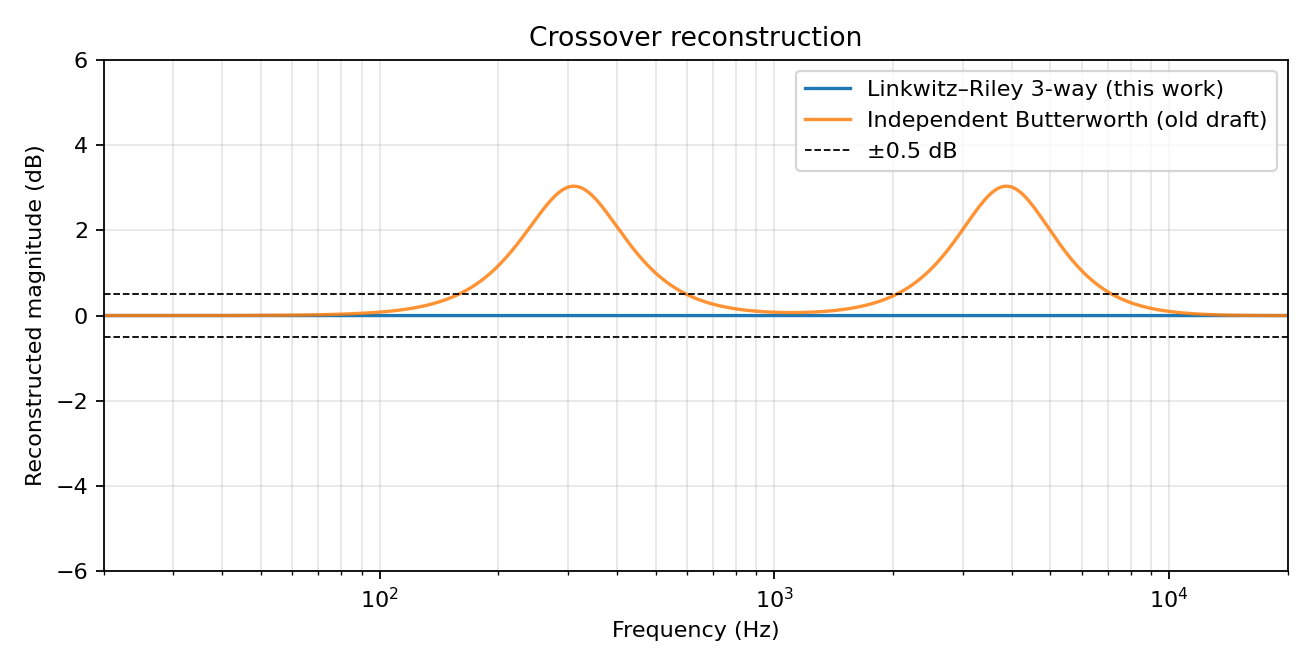
\includegraphics[width=\columnwidth]{crossover_reconstruction.png}
\caption{Crossover reconstruction. Linkwitz--Riley 3-way sum (this work) versus independent Butterworth splits used in an earlier draft. Dashed lines mark $\pm 0.5$\,dB.}
\label{fig:xo}
\end{figure}

\begin{figure}[!t]
\centering
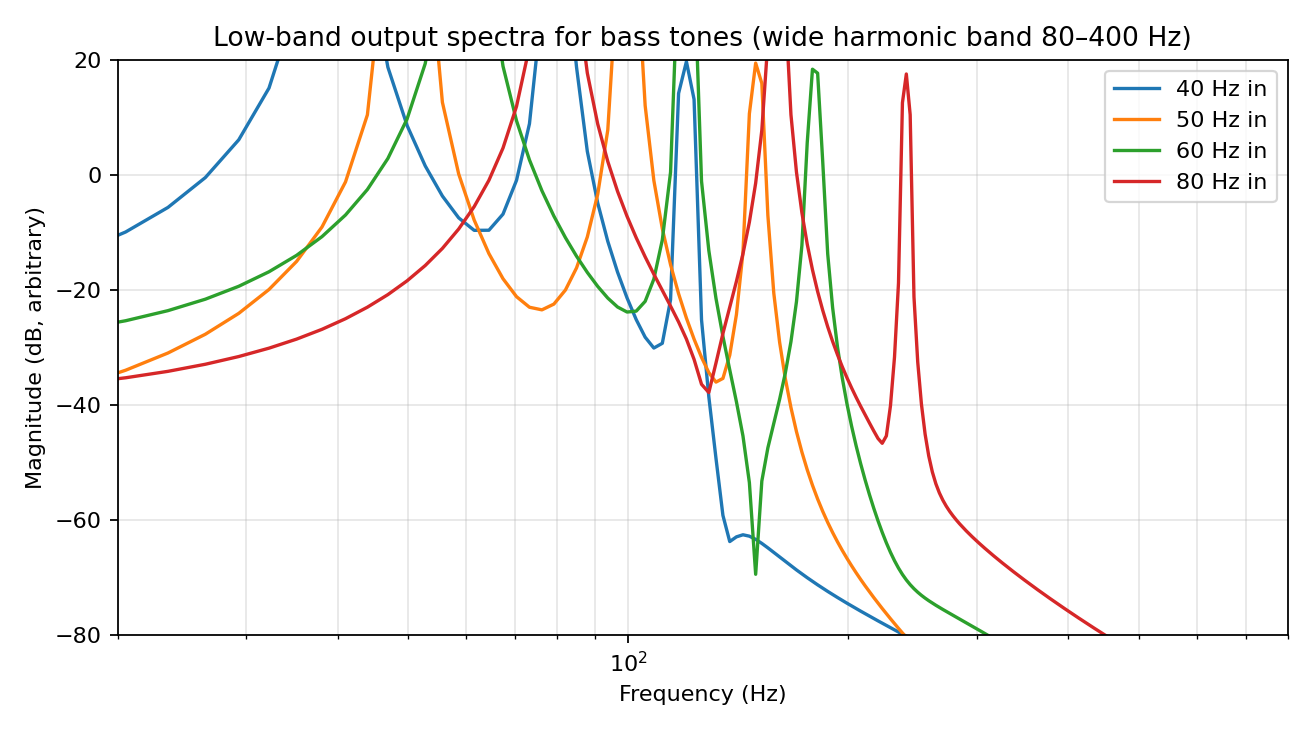
\includegraphics[width=\columnwidth]{harmonic_coverage.png}
\caption{Low-band output spectra for 40, 50, 60, and 80\,Hz tones after the $-12$\,dB shelf and 80--400\,Hz harmonic path. Second and third harmonics are present for a 40\,Hz fundamental.}
\label{fig:harm}
\end{figure}

\begin{figure}[!t]
\centering
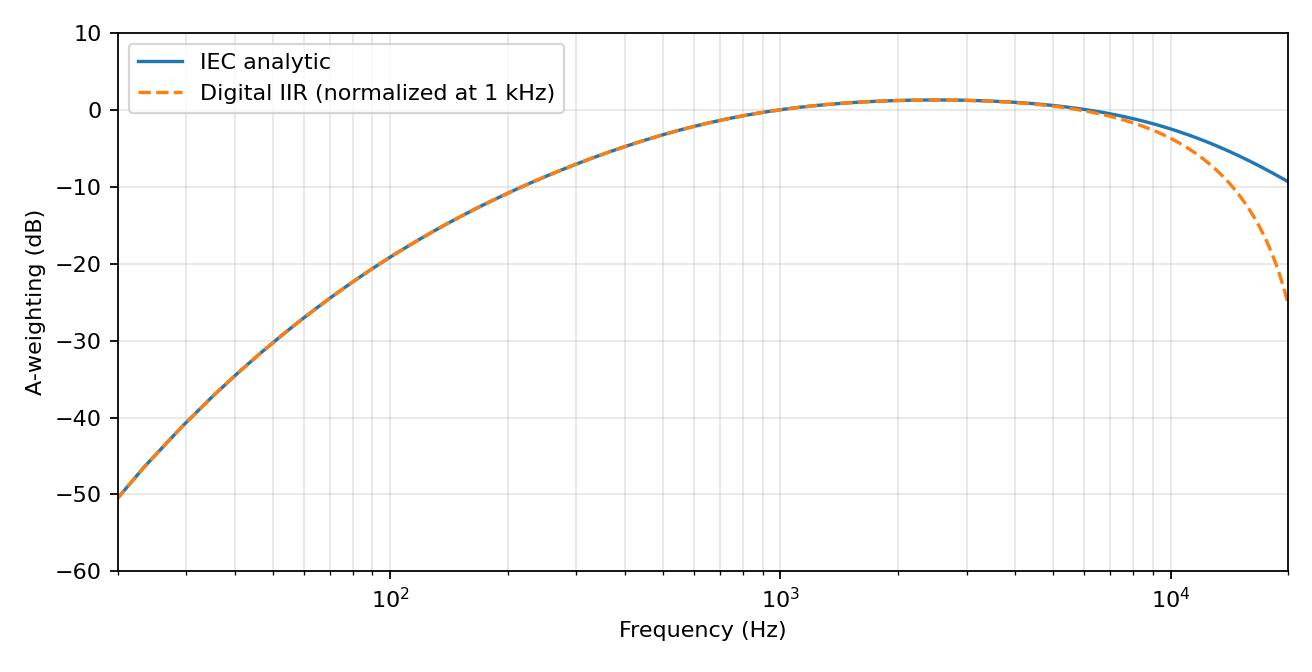
\includegraphics[width=\columnwidth]{aweighting_response.png}
\caption{Digital A-weighting IIR (normalised at 1\,kHz) versus the IEC analytic curve. The mid-band detector uses 300\,Hz--4\,kHz. A-weighting at 40\,Hz is about $-35$\,dB, which is the mechanism behind the main result.}
\label{fig:aw}
\end{figure}

\begin{figure}[!t]
\centering
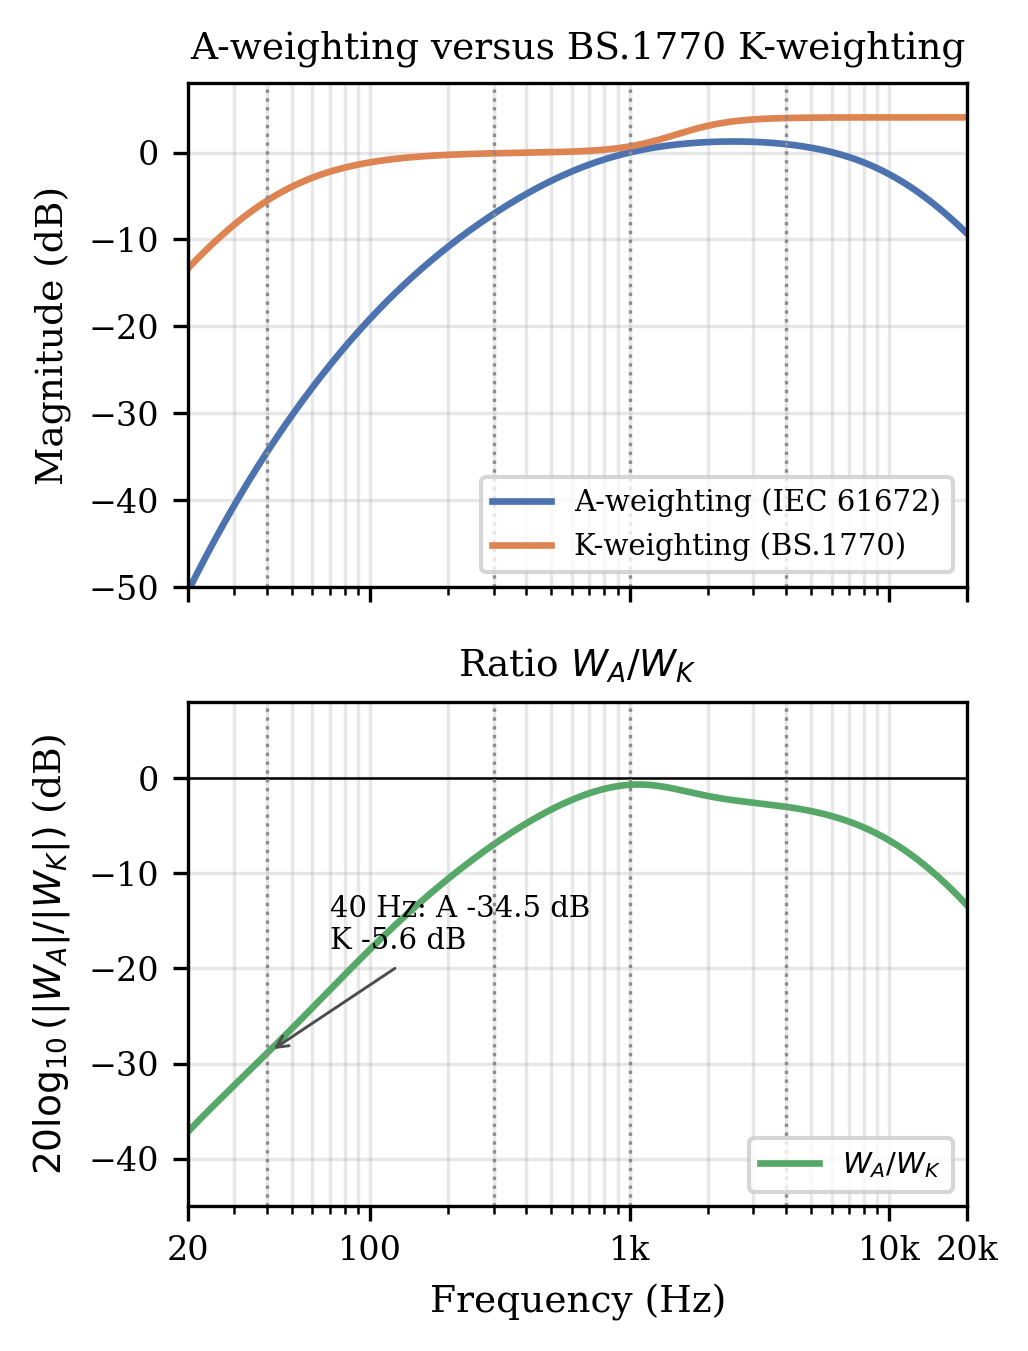
\includegraphics[width=\columnwidth]{weighting_ratio.png}
\caption{IEC A-weighting and BS.1770 K-weighting on the same axes, with the ratio $W_A/W_K$ in dB. Vertical markers: 40\,Hz, 300\,Hz, 1\,kHz, 4\,kHz. Near 40\,Hz, A-weighting is about $-35$\,dB while K-weighting is only a few dB down, so a bass cut spends loudness that the dose meter barely sees.}
\label{fig:wak}
\end{figure}

\section{Implementation}
\label{sec:impl}

The reference system is offline Python (\texttt{numpy}/\texttt{scipy}) at $f_s=48$\,kHz. All filters are causal: second-order sections with state carried across blocks. The processor is hop-based (256 samples) and streamable. Processing a 2\,s test signal in 240-sample blocks versus in one call gave a maximum absolute sample difference of 0.0. The output stage is a peak ceiling at $-1$\,dBFS; it never renormalises a quiet block back toward full scale.

Default parameters are listed in Table~\ref{tab:params}. Source code is the \texttt{exposure\_dsp} package in the project repository. Listings are omitted from the paper.

\begin{table}[!t]
\caption{Default processor parameters.}
\label{tab:params}
\centering
\renewcommand{\arraystretch}{1.12}
\begin{tabular}{l l}
\hline
Parameter & Value \\
\hline
Sample rate & 48\,kHz \\
Crossover & LR4, 300\,Hz / 4\,kHz \\
Sub-bass shelf $\beta$ & $-12$\,dB near 100\,Hz \\
Harmonic band & 80--400\,Hz ($a_2=0.8$, $a_3=0.35$) \\
Mid target / ratio & 78 / 4:1 \\
Mid attack / release & 5\,ms / 50\,ms \\
High threshold / $\gamma$ & $-12$\,dBFS / 0.5 \\
Output ceiling & $-1$\,dBFS \\
\hline
\end{tabular}
\end{table}

\section{Experimental Setup}
\label{sec:setup}

\subsection{Systems}

Every clip is processed by three systems:

\begin{enumerate}
\item \textbf{Original}: no processing.
\item \textbf{Frequency-flat gain}: one scalar $G$ applied to the whole waveform. This is the baseline that answers ``turn everything down.''
\item \textbf{Proposed}: the three-band processor of Section~\ref{sec:method} at the Table~\ref{tab:params} defaults.
\end{enumerate}

A secondary A-weighted broadband \emph{compressor} was also matched by searching its threshold. On many clips it never engaged, because the uncalibrated proxy never crossed the default target. Idle compression is not a fair ``turn it down'' baseline, so the reported comparison uses static flat gain.

\subsection{Matching}

Two matching rules are applied, each to within a few hundredths of a dB:

\begin{itemize}
\item \textbf{Matched exposure:} $G$ is chosen so the flat-gain output has the same digital $L_{Aeq}$ proxy as the proposed output.
\item \textbf{Matched loudness:} $G$ is chosen so the flat-gain output has the same integrated LUFS \cite{BS1770} as the proposed output (\texttt{pyloudnorm}).
\end{itemize}

Because flat gain is frequency-independent, both meters move by approximately $20\log_{10} G$. The two matching rules are therefore two views of one difference, not two independent experiments. The interesting content is the sign of that difference and which material produces it.

\subsection{Metrics}

The digital exposure proxy is A-weighted RMS plus an arbitrary offset,
\begin{equation}
L_{Aeq}^{\mathrm{proxy}} = 20\log_{10}\mathrm{RMS}\{w_A * x\} + 94.
\end{equation}
The offset 94 maps digital full scale to a convenient number for development. It is \emph{not} a calibration to pascals or to an ear simulator. Loudness is integrated LUFS. Spectral change versus the original is log-spectral distance (LSD) over Welch power estimates; LSD is an objective distance, not a listening-test score.

\subsection{Material}

The corpus has $n=20$ clips at 48\,kHz mono: 16 Creative Commons Freesound recordings (bass loops, drum loops, choir, solo vocal, speech, cymbals)\footnote{Freesound IDs 165523, 179270, 189635, 269906, 380303, 431525, 479941, 529808, 541260, 627643, 628213, 629137, 629139, 657761, 735157, 739037.} and four built-in synthetic programmes (bass-heavy, speech-like, transient, mixed). Synthetics are included for completeness and labelled as such. The conclusions below are also stated for the 16 real recordings alone.

\subsection{Hypotheses}

\begin{itemize}
\item \textbf{H2 (matched loudness):} at equal LUFS, the proposed $L_{Aeq}$ proxy is lower than flat gain.
\item \textbf{H1 (matched exposure):} at equal $L_{Aeq}$ proxy, the proposed output is louder (higher LUFS) and/or closer to the original in LSD.
\end{itemize}

\subsection{Listening notes}

No formal MUSHRA or PEAQ test was run, and no listener scores are reported. Processed files are available as \texttt{*_proposed.wav} versus \texttt{*_gain\_matched\_loudness.wav} (equal LUFS) and \texttt{*_gain\_matched\_exposure.wav} (equal proxy). A later test should lock playback volume, randomise order, and collect ratings for overall quality, bass, clarity, and loudness. Until that is done, quality claims stay with LUFS and LSD.

\section{Results}
\label{sec:results}

\subsection{Matched loudness: exposure proxy}

Fig.~\ref{fig:h2} plots, for each clip, the proposed digital $L_{Aeq}$ proxy minus the flat-gain proxy at matched LUFS. Positive bars mean the proposed system is \emph{worse} on the quantity it was supposed to reduce.

\begin{figure*}[!t]
\centering
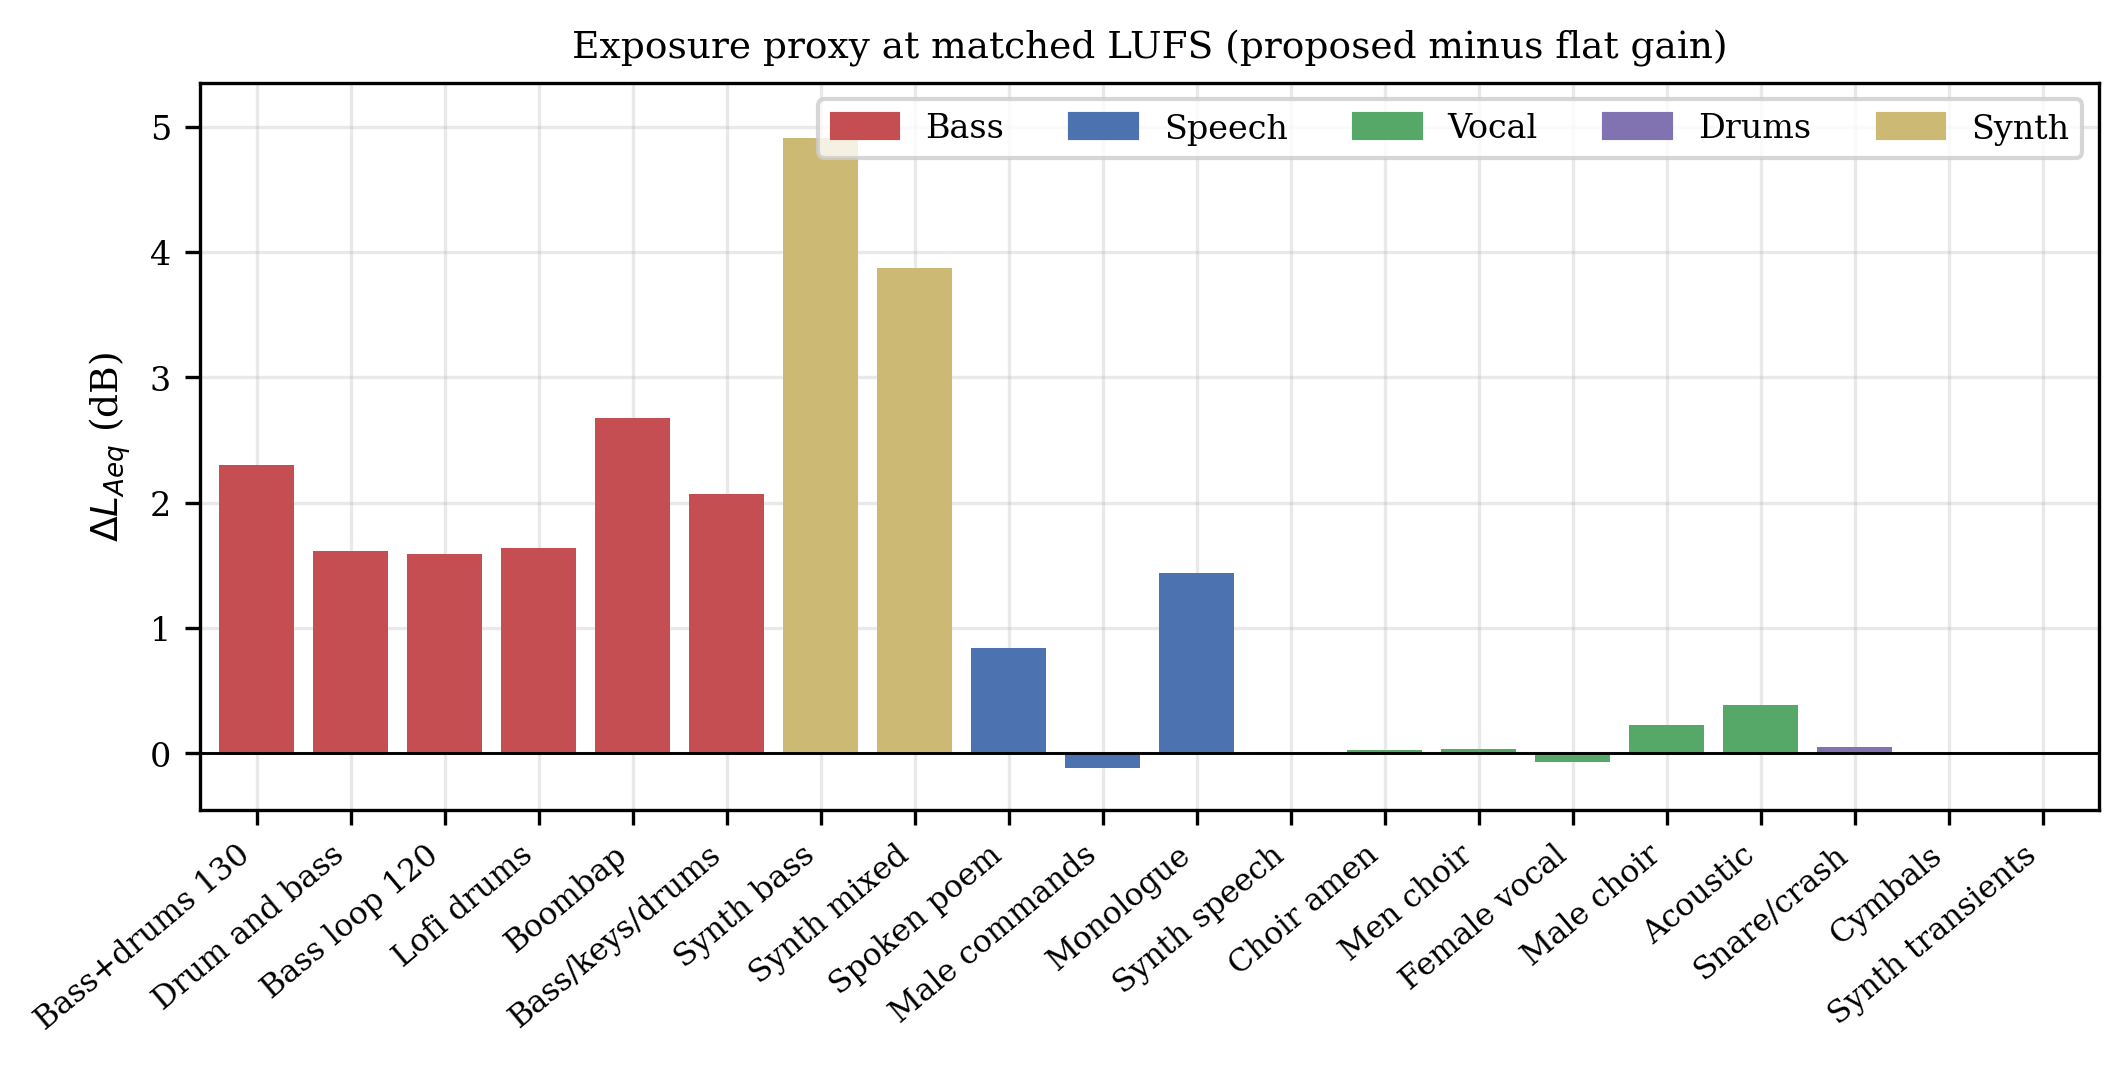
\includegraphics[width=\textwidth]{matched_loudness_delta.png}
\caption{Digital $L_{Aeq}$ proxy at matched LUFS: proposed minus frequency-flat gain. Positive values mean the proposed processor has the higher exposure proxy. Bass loops (red) drive the mean; speech, vocals, and short transients sit near zero.}
\label{fig:h2}
\end{figure*}

The mean over 20 clips is $+1.17$\,dB (median $+0.61$\,dB). On the 16 Freesound recordings alone the mean is $+0.92$\,dB. Twelve clips are more than 0.05\,dB worse for the proposed system, six are within 0.05\,dB, and two are slightly better (a female vocal at $-0.07$\,dB and mixed command speech at $-0.12$\,dB). \textbf{H2 is not supported.}

The failure is concentrated in bass. The six real bass and drum-loop clips sit between $+1.59$ and $+2.67$\,dB (mean $+1.98$\,dB). Speech, choir, solo vocal, and cymbal clips as a group average $+0.28$\,dB. Synthetic bass and mixed programmes are more extreme ($+4.91$ and $+3.87$\,dB) because they were built with strong 40--50\,Hz components; they inflate the overall mean but they do not create the finding. Real bass loops already go the same way.

Per-clip numbers are in Table~\ref{tab:perclip}. A Wilcoxon signed-rank test on the 20 $\Delta L_{Aeq}$ values rejects a zero median two-sided ($p=3.9\times 10^{-4}$; rank-biserial $r=0.84$). The one-sided test of H2 ($\Delta<0$) is not supported ($p\approx 1$). The bootstrap 95\% CI on the mean is $[0.60,\,1.83]$\,dB. On the 16 real recordings the mean is $+0.92$\,dB (CI $[0.47,\,1.39]$; two-sided $p=0.002$). The six real bass loops sit at $+1.98$\,dB (CI $[1.69,\,2.33]$).

\begin{table*}[!t]
\centering
\caption{Per-clip $\Delta L_{Aeq}$ at matched LUFS (processor minus flat gain; positive: higher digital exposure proxy) and the dual $\Delta$LUFS at matched $L_{Aeq}$. S1 is the bass-first heuristic; S2 is the metric-aligned mid cut.}
\label{tab:perclip}
\renewcommand{\arraystretch}{1.08}
\begin{tabular}{l l r r r r}
\hline
Clip & Type & $\Delta L_{Aeq}$ S1 & $\Delta L_{Aeq}$ S2 & $\Delta$LUFS S1 & $\Delta$LUFS S2 \\
\hline
Bass+drums 130 & Bass & +2.30 & -0.69 & -2.30 & +0.69 \\
Drum and bass & Bass & +1.61 & -0.96 & -1.61 & +0.96 \\
Bass loop 120 & Bass & +1.59 & -0.00 & -1.59 & +0.00 \\
Lofi drums & Bass & +1.63 & -1.08 & -1.63 & +1.08 \\
Boombap & Bass & +2.67 & -0.51 & -2.67 & +0.51 \\
Bass/keys/drums & Bass & +2.07 & -0.18 & -2.07 & +0.18 \\
Synth bass & Synth & +4.91 & +0.00 & -4.91 & -0.00 \\
Synth mixed & Synth & +3.87 & -0.35 & -3.87 & +0.35 \\
Spoken poem & Speech & +0.84 & -0.18 & -0.85 & +0.18 \\
Male commands & Speech & -0.12 & -1.19 & +0.12 & +1.18 \\
Monologue & Speech & +1.44 & -0.07 & -1.44 & +0.07 \\
Synth speech & Synth & +0.01 & -0.11 & -0.01 & +0.11 \\
Choir amen & Vocal & +0.03 & -0.02 & -0.03 & +0.02 \\
Men choir & Vocal & +0.04 & -0.01 & -0.04 & +0.01 \\
Female vocal & Vocal & -0.07 & -0.16 & +0.07 & +0.16 \\
Male choir & Vocal & +0.22 & -0.00 & -0.22 & +0.00 \\
Acoustic & Vocal & +0.38 & -0.03 & -0.38 & +0.03 \\
Snare/crash & Drums & +0.05 & +0.20 & -0.05 & -0.20 \\
Cymbals & Drums & -0.01 & +0.02 & +0.01 & -0.02 \\
Synth transients & Synth & +0.01 & -0.00 & -0.01 & +0.00 \\
\hline
Mean ($n$=20) &  & +1.17 & -0.27 & -1.17 & +0.27 \\
\hline
\end{tabular}
\end{table*}


\subsection{Why the proxy moves the wrong way}

Fig.~\ref{fig:mismatch} plots, for the proposed output versus the original, LUFS drop against $L_{Aeq}$ drop. If the two meters agreed, points would lie on the dashed line. Bass clips lie far to the right: LUFS falls by 2--5\,dB while the A-weighted proxy barely moves. Speech and cymbals lie near the origin.

\begin{figure}[!t]
\centering
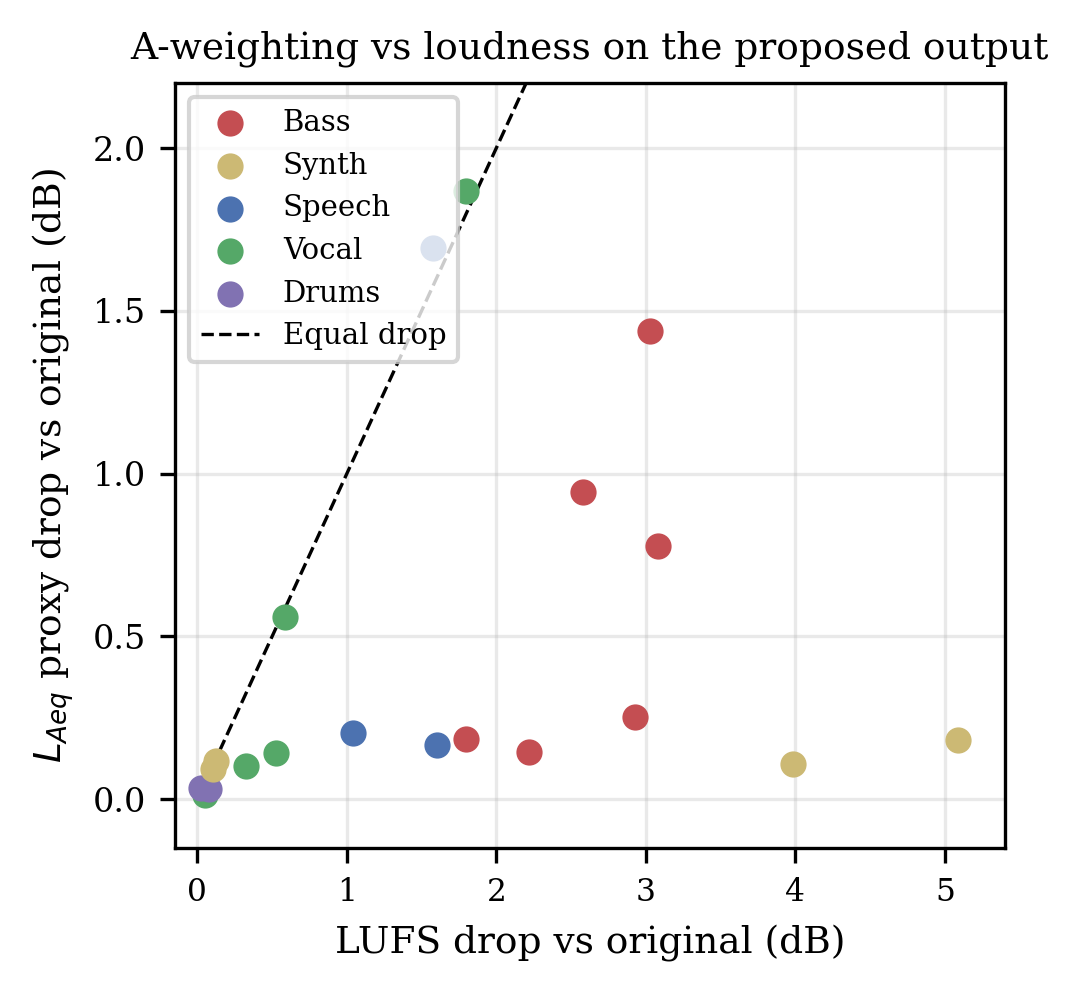
\includegraphics[width=\columnwidth]{metric_mismatch.png}
\caption{Proposed processor versus the original clip. Bass-heavy material loses loudness (LUFS) without a matching drop in the A-weighted proxy, because A-weighting already ignores energy near 40\,Hz.}
\label{fig:mismatch}
\end{figure}

A-weighting at 40\,Hz is approximately $-35$\,dB (Fig.~\ref{fig:aw}). BS.1770 K-weighting does not discount that region to the same degree (Fig.~\ref{fig:wak}). The low-band shelf therefore does what it was designed to do---remove sub-bass---and LUFS notices. The exposure proxy does not. To match LUFS, flat gain must apply that same loudness reduction to the \emph{whole} spectrum, including the midrange that A-weighting does count. Flat $L_{Aeq}$ therefore falls further. Frequency-selective allocation aimed at ``cheap'' bass cuts is the wrong allocation for an A-weighted objective.

This is not a crossover bug. Reconstruction is flat (Fig.~\ref{fig:xo}), harmonics are present at 40\,Hz (Fig.~\ref{fig:harm}), and block streaming matches whole-signal processing. The negative result is a metric mismatch, not an implementation failure.

\subsection{Matched exposure: loudness and spectral distance}

Fig.~\ref{fig:h1} is the dual view. At equal digital $L_{Aeq}$, the proposed output is quieter by 1.17\,dB LUFS on average---exactly the opposite sign of Fig.~\ref{fig:h2}, as expected for a frequency-flat baseline. \textbf{H1 is not supported as a loudness-preservation claim.} At the same A-weighted proxy, turning the whole signal down keeps more LUFS than cutting sub-bass.

\begin{figure*}[!t]
\centering
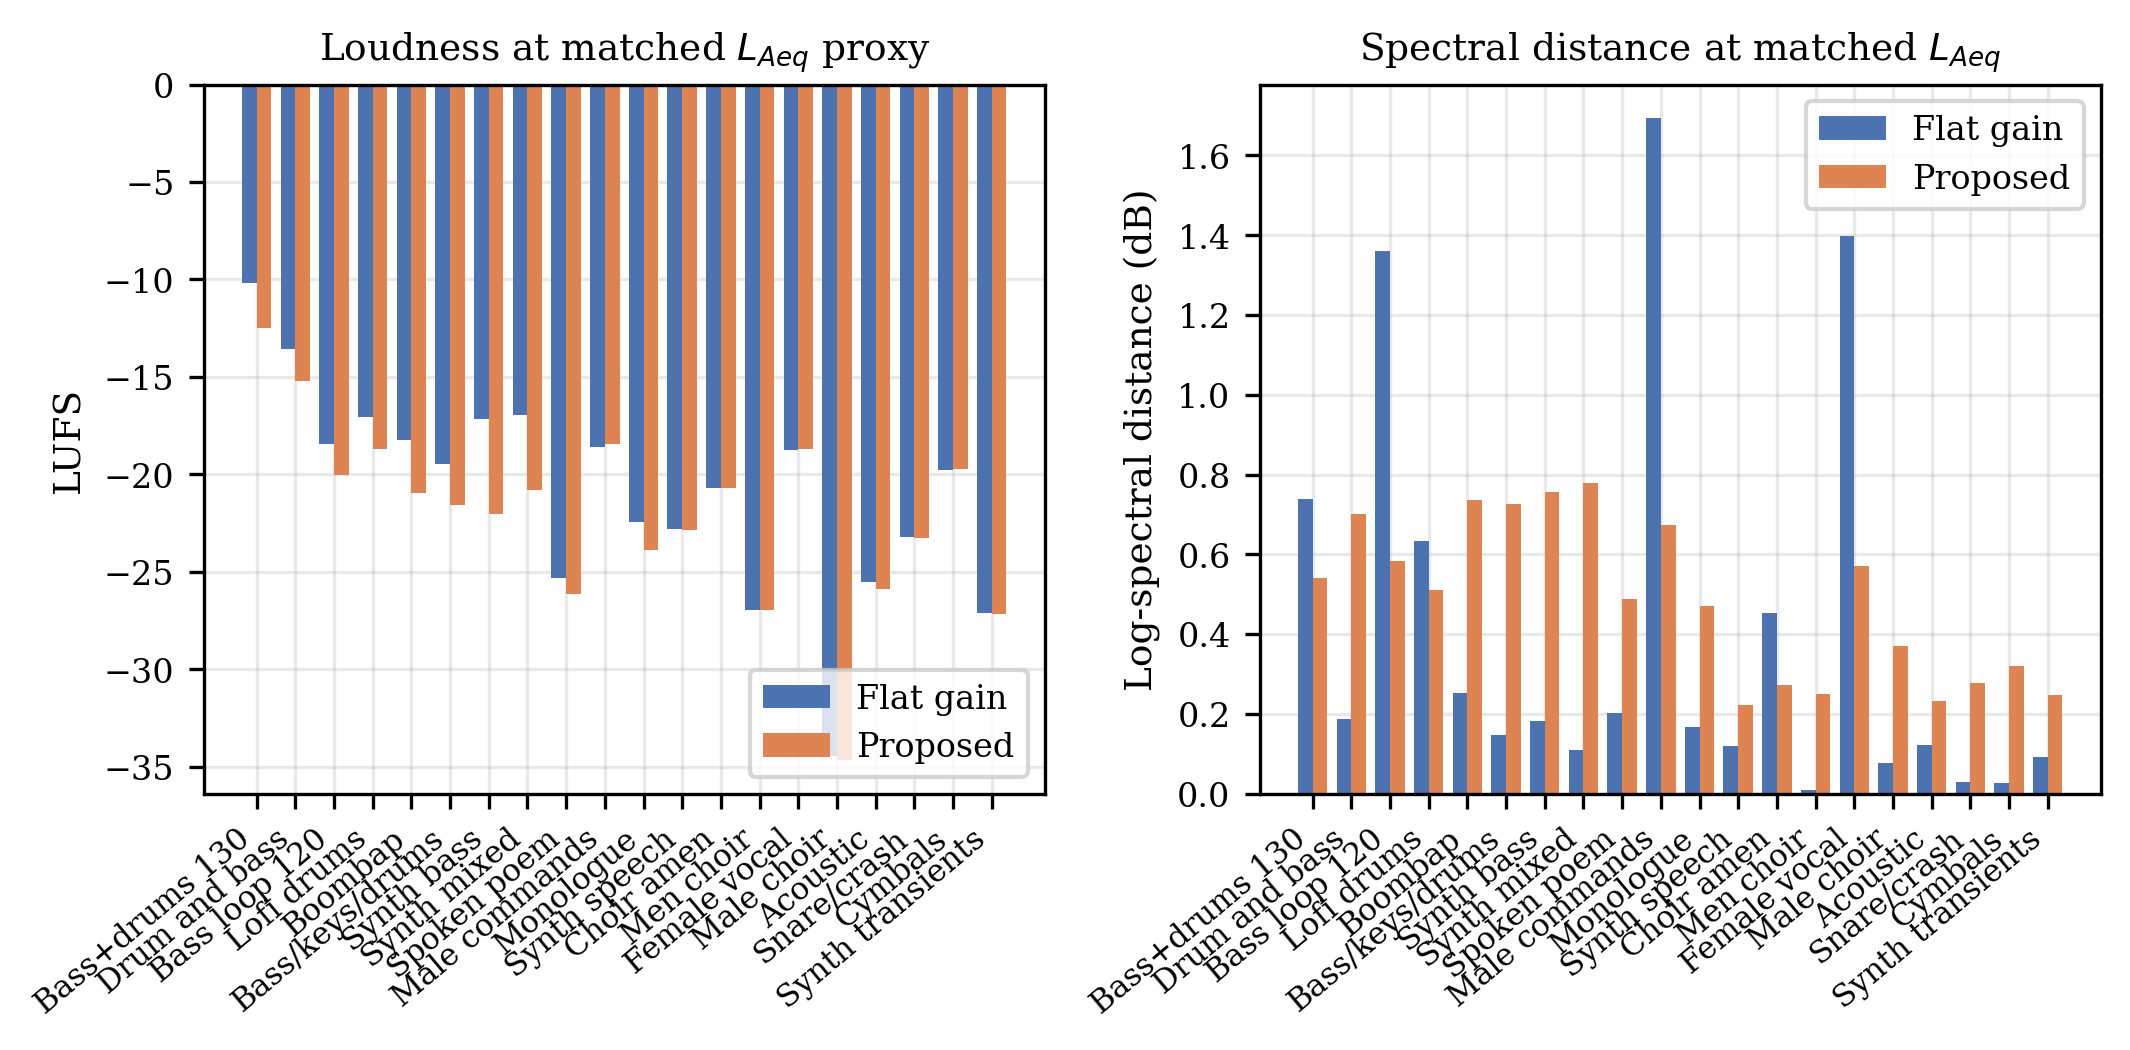
\includegraphics[width=\textwidth]{matched_exposure_quality.png}
\caption{Left: LUFS at matched digital $L_{Aeq}$ proxy. The proposed system is quieter on bass-heavy clips. Right: log-spectral distance versus the original at the same match. LSD is an objective distance, not a quality grade.}
\label{fig:h1}
\end{figure*}

Mean LSD is 0.49\,dB for the proposed system and 0.40\,dB for flat gain. On many bass clips flat gain barely moves, so its LSD is small. On clips where the mid-band compressor actually works (female vocal, command speech), flat gain of the same $L_{Aeq}$ drop produces a larger spectral shift than the band-limited compressor (LSD 1.40 and 1.69\,dB versus 0.57 and 0.67\,dB). Spectral distance is therefore mixed: the proposed system is not uniformly closer to the original, but it avoids the largest broadband shifts. Without a listening test that pattern should not be read as ``better quality.''

\subsection{Ablation}

Fig.~\ref{fig:abl} shows mean change versus the original when bands are enabled one at a time. Crossover-only reconstruction does not change level. Mid-only compression moves $L_{Aeq}$ on speech and vocals and does little on bass. Adding the low band is what drops LUFS. Adding the high band changes almost nothing on this corpus; transients in the test set rarely exceeded the high-band threshold. The full system tracks the mid+low curve. The exposure/loudness disagreement is produced by the low shelf, which is also the block that was supposed to be the advantage.

\begin{figure}[!t]
\centering
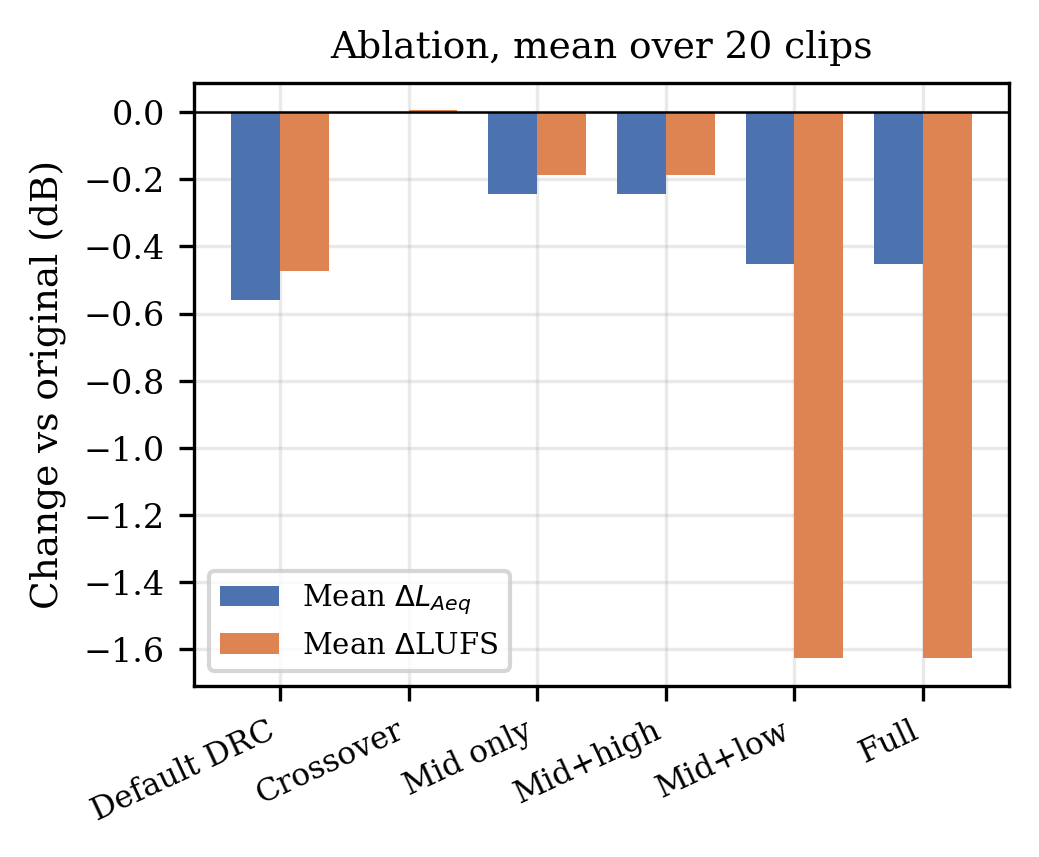
\includegraphics[width=\columnwidth]{ablation_delta.png}
\caption{Ablation, mean over 20 clips, relative to the unprocessed signal. ``Default DRC'' is a full-band A-weighted compressor at the default target, not the LUFS-matched flat gain of Fig.~\ref{fig:h2}. The low band dominates the LUFS drop. The high band is nearly unused on this material.}
\label{fig:abl}
\end{figure}

\subsection{Mid-band operating point}

A target/ratio sweep on a six-tone-plus-noise debug signal (Table~\ref{tab:sweep}) shows the expected trade-off: a lower mid target reduces the proxy and raises LSD. That sweep characterises the compressor. It is not the main result and it is not a perceptual quality measurement.

\begin{table}[!t]
\caption{Mid-band target/ratio sweep on a synthetic six-tone-plus-noise signal. $\Delta L_{Aeq}$ is versus the unprocessed debug clip. LSD is not a listening-test score.}
\label{tab:sweep}
\centering
\renewcommand{\arraystretch}{1.1}
\begin{tabular}{c c r r r}
\hline
Target & Ratio & $L_{Aeq}$ proxy & $\Delta L_{Aeq}$ (dB) & LSD (dB) \\
\hline
82 & 2:1 & 77.77 & $-0.10$ & 0.82 \\
80 & 3:1 & 77.77 & $-0.10$ & 0.82 \\
78 & 4:1 & 77.04 & $-0.83$ & 0.88 \\
76 & 4:1 & 75.92 & $-1.96$ & 1.16 \\
74 & 6:1 & 74.57 & $-3.30$ & 1.65 \\
72 & 8:1 & 73.34 & $-4.53$ & 2.20 \\
\hline
\end{tabular}
\end{table}

\section{Limitations}
\label{sec:limits}

This study compares two digital processing rules. It does not show prevention of hearing loss, and it does not report ear-level SPL. The $L_{Aeq}$ figures use an uncalibrated offset; a real mapping would require a specific earphone, volume setting, and an IEC~60318-4 occluded-ear simulator \cite{IEC60318}, which still is not an individual human ear.

LUFS is a standard loudness meter, not a booth loudness match. Band edges, shelf depth, and compressor constants were not searched over listeners. No Zwicker or Moore--Glasberg model is in the loop. No PEAQ or MUSHRA scores were collected. The high band did little on this set, so the experiment mainly contrasts a low-shelf-plus-harmonics path with flat gain. Four synthetic clips are in the mean; removing them lowers the matched-loudness gap from 1.17\,dB to 0.92\,dB and does not reverse the sign.

\section{Conclusion}
\label{sec:conclusion}

We asked whether a three-band, perceptually motivated limiter could reduce a digital A-weighted exposure proxy more than turning the whole signal down, at the same LUFS. On 20 clips it did not: the proposed proxy was 1.17\,dB higher on average, and 1.6 to 2.7\,dB higher on real bass loops. Vocals, speech, and short transients were a tie. Cutting sub-bass spends loudness on a band that A-weighting already ignores, so a flat gain that matches LUFS wins on $L_{Aeq}$. The useful outcome is that comparison. If an A-weighted dose limit is the constraint, frequency-selective bass cuts are a poor allocation; any later design should spend attenuation where $w_A(f)$ is large, or replace A-weighting with a metric that actually tracks the intended risk. Calibrated ear-simulator measurements and a locked-volume listening test remain the next experimental step.

\bibliographystyle{IEEEtran}
\bibliography{references}

\end{document}
